\section{Computer Program Optimization} \label{app:opt}

When optimizing a program, there is an important cardinal rule to follow which at times
is easy to forget in the face of increasingly interesting and complex minor optimizations
designed to squeeze every bit of performance out of your computer. Unfortunately, due
to the complexity of modern computer hardware, it is
very difficult to predict if a given micro-optimization will actually be benificial or
not. For this reason, the most important rule when taking a working program and making it
fast is\footnote{besides \textit{don't break it}, of course. An incorrect program is worthless, no matter
how fast it is.} \textit{benchmark everything}.

The field of program optimization is huge. There is a small number of people who, for
a given platform, are really \textit{good} at optimization. There is an even smaller number
who are truly experts. I do not fit into either of these categories. For this reason, the program
that I have written here is \textit{decently} optimized. I believe that the maximum throughput
is not orders of magnitude better than what I have achieved, however, there is still a lot of work
that can be done (including a potentially significant optimization that I have neglected, and will talk
about later).

%%%%%%%%%%%%%%%%%%%%%%%%%%%%%%%%%%%%%%%%%% ACTUALLY TALK ABOUT THAT ************************

\subsection{Freebies}

There are some optimizations which can be used in high confidence and are also very easy to do.
The first, and most obvious, is to use a fast language. While writing in \texttt{C} may be a chore
compared to writing in python, the resulting code will be much faster. This is the reason behind the
organization of this program: the frontend (which has no performance requirements) is written in
python because parsing the configuration file is much easier. The backend needs to be fast, so it
is implemented in \texttt{C}.

A quick and rough experiement can easily convince you that this is true (remember how I said to
benchmark everything?). Credit to my friend Chris Milke for doing this test. Write the following
code in both python and in C: initialize a variable to zero. Then loop from zero to some large
number (we used 123,456,789), and add that iteration to the variable. After the loop, print the
variable. The resultant python program took 14.25 seconds to run on my computer, but the C code
completed \textit{instantaneously}. Why is python slower than C in general? Because python is
an interpreted language. The code that you write is read by another program and executed by
that program. In contrast, C code must be compiled into machine code. This is then run directly
on the processor, which cuts out the middle-man of the interpreter.

When using C, there are some more things that you can get for free: compiler optimizations. When
compiling a C program, the command looks something like this: \texttt{gcc -Wall -Wextra foo.c}\footnote{as an aside, you should \textbf{always} compile with -Wall and -Wextra, and eliminate all warnings from your program.
Warnings are warnings for a reason, and should rarely be ignored.}. This will
result in a compiled C program (a binary file, containing the machine code), but it will be
unoptimized. There are reasons why one may want an unoptimized binary (they are typically
easier to debug, for example), but generally when you compile your program for actual usage
you will want to optimize it. An aggressive optimization compilation command may look something
like: \texttt{gcc -Wall -Wextra -O3 -ffast-math -mavx}, as a start. The main flag here is \texttt{-O3}, which
enables almost every optimization that gcc can do.

Going back to the example from earlier, the optimized version of the C program completed instantly, but
the unoptimized version took 0.33 seconds. The unoptimized version is still 43 times faster than the
python code, but what was the optimizing compiler doing to make it so much faster with \texttt{-O3} on?
Part of optimizing is understanding why something is faster, so lets look at the assembly code. On \textsc{unix},
this can be done with the objdump command. Table \ref{table:assem-1} shows the annotated assembly from
the function \texttt{main}. If you don't know x86\_64 assembly language, you will at least notice that the
optimized version is much shorter. If you do know how to read the assembly, you'll notice that the unoptimized
version is doing almost literally what the C code says to do: set a variable to zero, and iterate from zero to
a big number, adding that iteration to the variable, and finally printing the variable. The optimized code just prints a large number -- which happens to be the result of the sum.

\begin{table}[h]
	\centering
\begin{tabular}{l | l}
	\hline
	\textbf{Unoptimized} & \textbf{Optimized}\\
	\hline
	\texttt{mov [rbp-0x10], 0x0}	&\texttt{movabs rsi,0x1b131147ee6b52} \\
	\texttt{jmp .loop\_end			}	&\texttt{mov edi,0x400594} \\
	\texttt{.loop\_top:                } &\texttt{xor eax,eax   } \\
	\texttt{mov rax, [rbp-0x10]				}	&\texttt{jmp 4003c0 <printf@plt>}\\
	\texttt{add [rbp-0x8], rax				}	&\texttt{	} \\
	\texttt{add [rbp-0x10], 0x1				}	&\texttt{ }\\	
	\texttt{.loop\_end:                       } &\texttt{} \\
	\texttt{cmp [rbp-0x10],0x75bcd14} &\texttt{} \\
	\texttt{jle loop\_top} &\texttt{} \\
	\texttt{mov rsi,[rbp-0x8]} &\texttt{} \\
	\texttt{mov edi, 0x4005b4} &\texttt{} \\
	\texttt{mov eax, 0} &\texttt{} \\
	\texttt{call 4003c0 <printf@plt>} &\texttt{} \\
\end{tabular}
	\caption{Unoptimzed and optimized assembly from the sum-a-lot-of-numbers example.}
	\label{table:assem-1}
\end{table}

This is just a simple example, but a good C compiler can drastically improve the performance of a
program. Here, it made a program that took a third of a second (which is already drastically faster than
the interpreted python version!) finish instantly.

\subsection{A Model of Processor Design}



\begin{figure}[h]
\begin{subfigure}{0.4\textwidth}
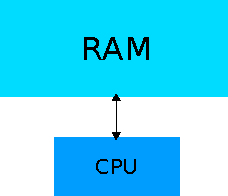
\includegraphics[width=\linewidth]{ram-cpu-simple.pdf}
\caption{Simplistic view of CPU and RAM.} \label{fig:1a}
\end{subfigure}
\hfill
\begin{subfigure}{0.4\textwidth}
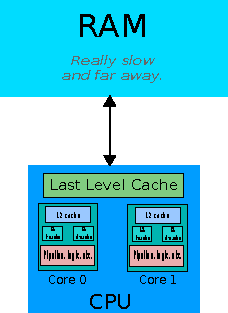
\includegraphics[width=\linewidth]{ram-cpu-complex.pdf}
\caption{More realistic view of CPU and RAM.} \label{fig:1b}
\end{subfigure}
\label{fig:cpu-and-ram}
\caption{View of programming that programmers like to have (a), versus the the more realistic
and complicated view.}
\end{figure}


\subsection{Structure of Arrays}

\subsection{Multithreading}

\subsection{Vectorization}
\subsubsection{Branch Reduction}



